\documentclass{article}

% Language setting
% Replace `english' with e.g. `spanish' to change the document language
\usepackage[UTF8]{ctex}

% Set page size and margins
% Replace `letterpaper' with `a4paper' for UK/EU standard size
\usepackage[letterpaper,top=2cm,bottom=2cm,left=3cm,right=3cm,marginparwidth=1.75cm]{geometry}

% Useful packages
\usepackage{amsmath}
\usepackage{amsfonts,amssymb}
\usepackage{bm}
\usepackage{graphicx}
\usepackage[colorlinks=true, allcolors=blue]{hyperref}

\title{多元函数入门攻略(下)}
\date{}
\author{Author:洛}

\begin{document}
\maketitle


本文主要讲述多元函数(以2个自变量的函数为例)极限、可微、连续、偏导数和方向导数之间的关系以及做题方法。分为以下5个部分:概述、定义、常见题型、反例、总结。



\tableofcontents

\newpage
\setcounter{page}{1}

\section{概述}
见多元函数入门攻略(上)

\section{定义}
见多元函数入门攻略(上)

\section{常见题型及方法}
见多元函数入门攻略(上)

\section{反例}
\begin{figure}[!h]
    \centering
    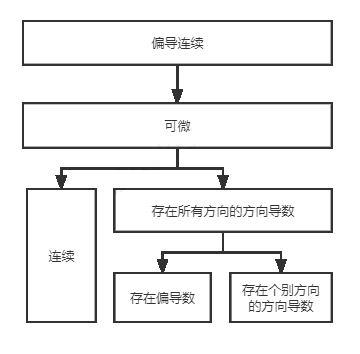
\includegraphics[width=0.5\textwidth]{pic/01.png}
    \caption{关系图}
\end{figure}

我们在概述中也见过这个关系图,图中沿箭头指向方向是恒成立的(比如:偏导函数连续一定能得到可微),但是没有标注箭头的是不恒成立的,下面会举出这些不成立的反例并证明。

\subsection{可微不能推出偏导连续}
举出一个可微,但偏导不连续的反例:

\textbf{反例1}:f在原点可微,但$\frac{\partial f}{\partial x} $和$\frac{\partial f}{\partial y} $在原点不连续
\[f(x,y)= \begin{cases} (x^2+y^2)sin \frac{1}{x^2+y^2}   & (x,y) \neq (0,0)\\0 & (x,y) = (0,0)\end{cases}\]

证明:先用定义求出$\frac{\partial f(0,0)}{\partial x}$和$\frac{\partial f(0,0)}{\partial y}$
\[\frac{\partial f(0,0)}{\partial x}=  \lim\limits_{x \rightarrow 0} \frac{f(x,0)-f(0,0)}{x}=\lim\limits_{x \rightarrow 0} \frac{0-0}{x}=0\]
同理,
\[\frac{\partial f(0,0)}{\partial y}=  \lim\limits_{y \rightarrow 0} \frac{f(0,y)-f(0,0)}{y}=\lim\limits_{y \rightarrow 0} \frac{0-0}{y}=0\]
要证明原点处的可微性,由定义即证明
\[\lim\limits_{(x,y) \rightarrow (0,0)} \frac{ f(x,y)-f(0,0) - \frac{\partial f}{\partial x}(0,0) x - \frac{\partial f}{\partial y}(0,0) y}{ \sqrt{x^2 + y^2} } = 0\]
化简后即证明
\[\lim\limits_{(x,y) \rightarrow (0,0)} \sqrt{x^2 + y^2}sin \frac{1}{x^2+y^2} = 0\]
换元$x=rcos\theta$,$y=rsin\theta$
\[\lim\limits_{(x,y) \rightarrow (0,0)} \sqrt{x^2 + y^2}sin \frac{1}{x^2+y^2}
=\lim\limits_{r \rightarrow 0} rsin\frac{1}{r^2} = 0\]
最后一个等号成立是因为,$r$是无穷小,$sin\frac{1}{r^2}$有界(正弦函数值域为$\left[-1,1\right]$),有界乘无穷小是0(回顾一下高数上/数分1)\\
至此,在原点的可微性得证。
当$(x,y) \leq (0,0)$时,直接求偏导有
\[\frac{\partial f}{\partial x}(x,y)=2x\left(sin \frac{1}{x^2+y^2} - \frac{1}{x^2+y^2}cos\frac{1}{x^2+y^2}\right) \]
当$(x,y) = (0,0)$时,上面求得,$\frac{\partial f}{\partial x}(0,0)=0$\\
判断是否连续,只需要判断函数在原点的极限值是否等于原点的函数值(也就是0)\\
使用极坐标换元可以得出(这里不展示详细过程了),下列极限不存在
\[\lim\limits_{(x,y) \rightarrow (0,0)} \frac{\partial f}{\partial x}(x,y) \]
因此$\frac{\partial f}{\partial x}$在原点不连续。同样的,$\frac{\partial f}{\partial y}$在原点也不连续。

\begin{figure}[!h]
    \centering
    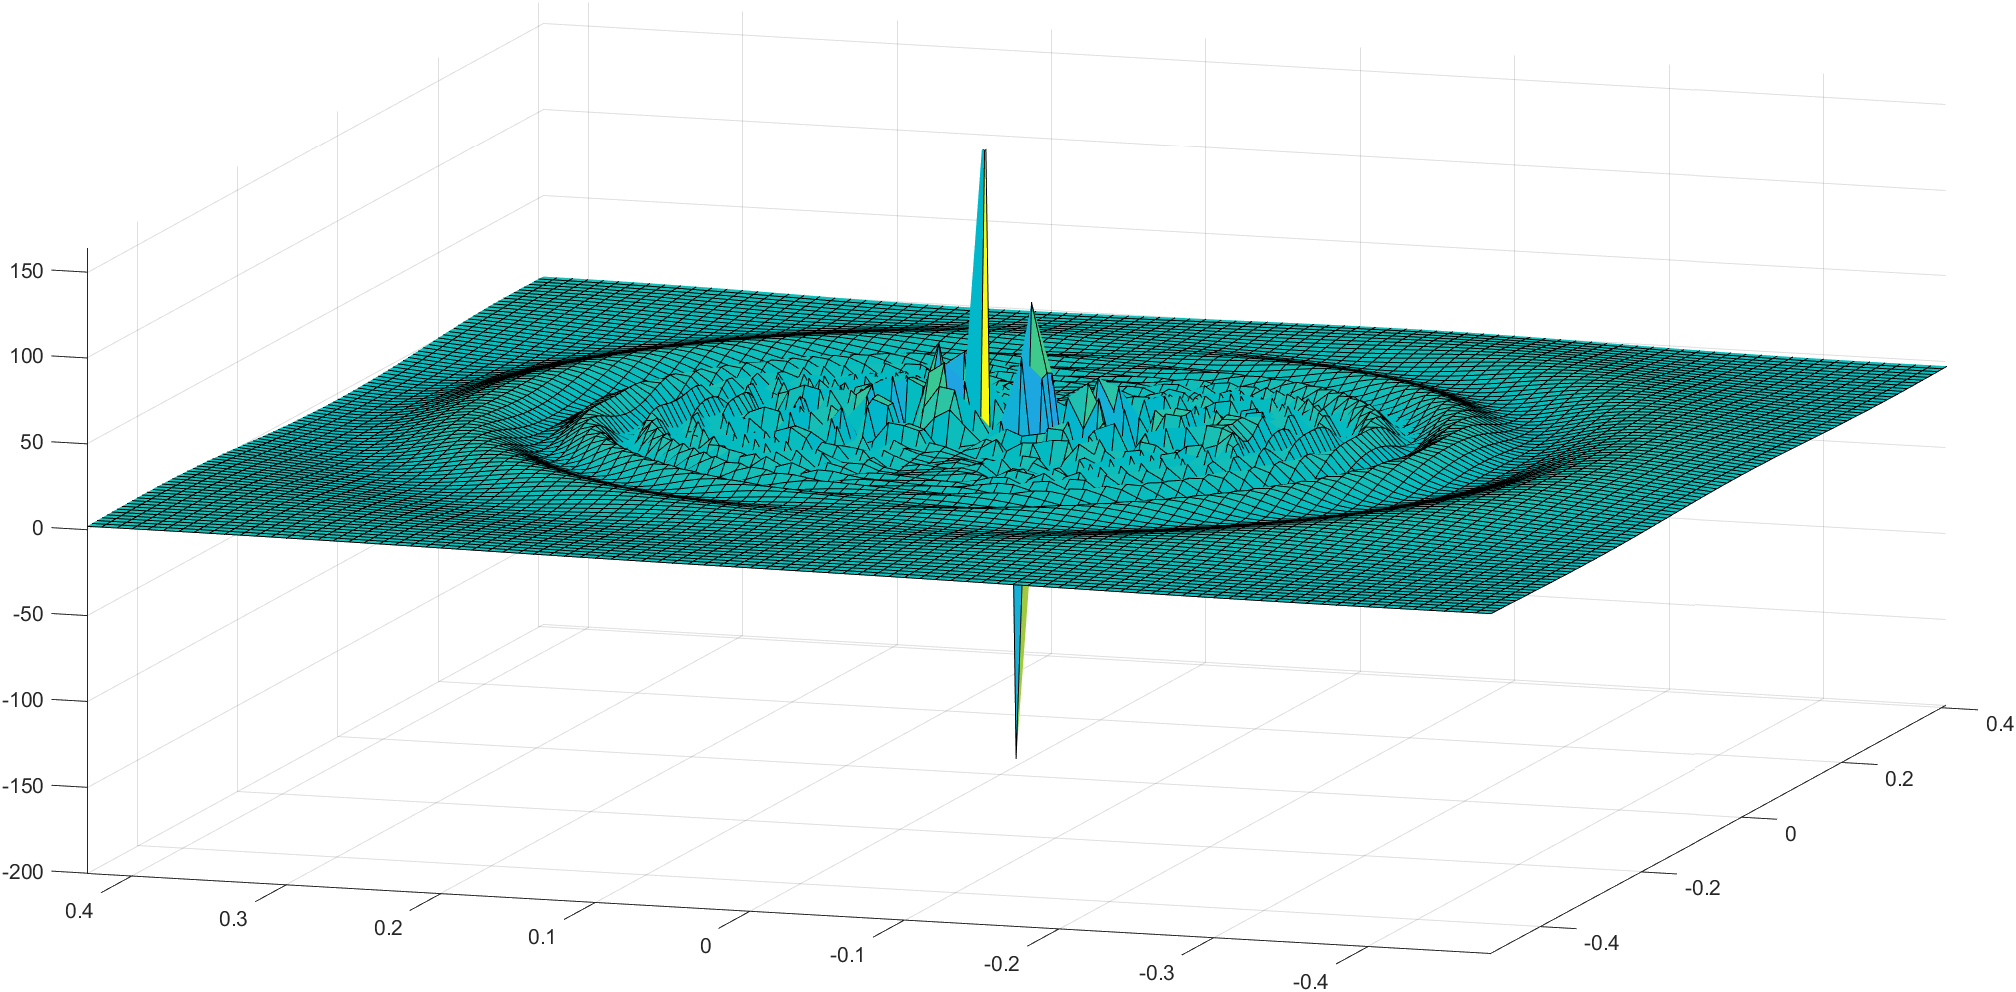
\includegraphics[width=0.6\textwidth]{pic/02.png}
    \caption{}
\end{figure}

如果参考上图,也许能更好的理解$\frac{\partial f}{\partial y}$在原点不连续这件事

\newpage

\subsection{仅存在偏导数,不存在方向导数也不连续}
\begin{figure}[!h]
    \centering
    
\includegraphics[width=0.35\textwidth]{pic/03.png}
    \caption{本情况满足关系图中的条件}
\end{figure}

\textbf{反例2}:f在原点存在偏导数,不存在方向导数,在原点不连续
\[f(x,y)= \begin{cases} \frac{xy}{x^2+y^2}   & (x,y) \neq (0,0)\\0 & (x,y) = (0,0)\end{cases}\]

证明:换元$x=rcos\theta$,$y=rsin\theta$,可得
\[\lim\limits_{(x,y) \rightarrow (0,0)} f(x,y) =\lim\limits_{r \rightarrow 0} \frac{r^2sin\theta cos\theta}{r^2}=sin\theta cos\theta\]
结果与$\theta$有关,因此$f$趋于原点极限不存在,\textbf{所以在原点不连续}。\\
直接使用定义求偏导数:
\[\frac{\partial f(0,0)}{\partial x}=  \lim\limits_{x \rightarrow 0} \frac{f(x,0)-f(0,0)}{x} = \lim\limits_{x \rightarrow 0} \frac{0-0}{x}=0\]
同样的,
\[\frac{\partial f(0,0)}{\partial y} = 0\]
\textbf{因此偏导数存在}\\
要证明其他方向导数不存在,先设方向$\mathbf{u}=(cos\theta,sin\theta)$,其中$\theta \neq 0,\frac{\pi}{2},\pi,\frac{3\pi}{2}$,因为$\mathbf{u}$不同于x、y方向(否则就是偏导数了)\\
利用方向导数的定义计算在原点的方向导数:
\[\frac{\partial f}{\partial \mathbf{u}}(0,0) =\lim\limits_{t \rightarrow 0^+} \frac{f(tcos\theta,tsin\theta)-f(0,0)}{t}=\lim\limits_{t \rightarrow 0^+} \frac{sin\theta cos\theta}{t}\]
$sin\theta cos\theta \neq 0$,因此极限不存在,\textbf{即方向导数不存在}

\newpage

\subsection{仅存在个别方向的方向导数,不存在偏导数也不连续}
\begin{figure}[!h]
    \centering
    
\includegraphics[width=0.35\textwidth]{pic/04.png}
    \caption{本情况满足关系图中的条件}
\end{figure}

\textbf{反例3}:f在原点存在某个方向的方向导数,不存在偏导数,在原点不连续
\[f(x,y)= \begin{cases} \frac{xy}{x^2+y^2}   & (x,y) \neq (0,0)\\ \frac{1}{2}& (x,y) = (0,0)\end{cases}\]

证明:在反例2中已经证明过,f在原点出极限不存在,\textbf{因此不连续}\\
由定义求在f在原点的偏导数
\[\frac{\partial f(0,0)}{\partial x}=  \lim\limits_{x \rightarrow 0} \frac{f(x,0)-f(0,0)}{x} = \lim\limits_{x \rightarrow 0} \frac{0-\frac{1}{2}}{x}\]
极限不存在,\textbf{因此没有对x的偏导数。同样的,也没有对y的偏导数}\\
考虑方向$\mathbf{u}=(\frac{\sqrt{2}}{2},\frac{\sqrt{2}}{2})$,由定义求在原点f对$\mathbf{u}$的方向导数
\[\frac{\partial f(0,0)}{\partial \mathbf{u}}=  \lim\limits_{t \rightarrow 0} \frac{f(t\mathbf{u})-f(0,0)}{t} = \lim\limits_{t \rightarrow 0} \frac{\frac{1}{2}-\frac{1}{2}}{x}=0\]
\textbf{因此存在该方向的方向导数。}不过容易验证,$-\mathbf{u}$方向也存在方向导数,并且也为0

~\\

对比反例2和反例3可以发现,仅仅是原点的值不同,存在方向导数的方向就不相同。这种现象可以理解为,在函数图像上,临近原点处会变得非常陡峭,因此原点处的取值不同,和临近原点处能连接在一起的方向就会改变,也就是每个原点处的函数值会对应几个方向有方向导数

\newpage


\subsection{存在偏导数和个别方向的方向导数,不存在全部方向导数也不连续}
\begin{figure}[!h]
    \centering
    
\includegraphics[width=0.35\textwidth]{pic/05.png}
    \caption{本情况满足关系图中的条件}
\end{figure}

这种情况大致上是上面两种情况的结合,有部分方向有方向导数,这些方向也包含x和y方向。这里给出一个反例,但严格证明的过程略去了【证明方法可以参考多元函数入门攻略(上)】

\textbf{反例4}:f在原点存在某个方向的方向导数和偏导数,不存在全部方向导数,在原点不连续
\[f(x,y)= \begin{cases} \frac{x^2y}{x^4+y^2}+\frac{xy}{\sqrt{x^2+y^2}}   & (x,y) \neq (0,0)\\ 0 & (x,y) = (0,0)\end{cases}\]


\subsection{存在全部方向的方向导数但不连续}
\begin{figure}[!h]
    \centering
    
\includegraphics[width=0.35\textwidth]{pic/06.png}
    \caption{本情况满足关系图中的条件}
\end{figure}

\textbf{反例5}:f在原点存在全部方向导数包含偏导数,但在原点不连续
\[f(x,y)= \begin{cases} \frac{x^2y}{x^4+y^2}   & (x,y) \neq (0,0)\\ 0 & (x,y) = (0,0)\end{cases}\]

\newpage
证明:设$y=kx^2$,可以得到f趋近于原点极限不存在,\textbf{因此不连续}\\
设方向$\mathbf{u}=(x,kx)$,由方向导数定义
\[\frac{\partial f(0,0)}{\partial \mathbf{u}}=  \lim\limits_{x \rightarrow 0} \frac{f(x,kx)-f(0,0)}{x} =  \lim\limits_{x \rightarrow 0} \frac{kx}{x^2+k^2} = 0\]
\textbf{因此任意方向均存在方向导数},为0


\subsection{连续,不存在方向导数及偏导数}
\begin{figure}[!h]
    \centering
    
\includegraphics[width=0.35\textwidth]{pic/07.png}
    \caption{本情况满足关系图中的条件}
\end{figure}

\textbf{反例6}:f在原点连续,但不存在方向导数包含偏导数
\[f(x,y)= \sqrt[3]{x^2+y^2} \]

证明:f在原点处依旧是初等函数,没有被表示成分段函数,\textbf{因此连续}\\
设方向$\mathbf{u}=(cos\theta,sin\theta)$,根据方向导数的定义求原点处的方向导数
\[\frac{\partial f(0,0)}{\partial \mathbf{u}}=  \lim\limits_{t \rightarrow 0} \frac{f(tcos\theta,tsin\theta)-f(0,0)}{t} = \lim\limits_{t \rightarrow 0} t^{-\frac{1}{3}}\]
极限不存在,\textbf{因此任意方向的方向导数(含偏导数)均不存在}

\newpage

\subsection{连续且存在偏导数,不存在其他方向导数}
\begin{figure}[!h]
    \centering
    
\includegraphics[width=0.35\textwidth]{pic/08.png}
    \caption{本情况满足关系图中的条件}
\end{figure}

\textbf{反例7}:f在原点连续且有偏导数,但不存在其他任何方向导数
\[f(x,y)= \begin{cases}  \sqrt[3]{x^2+y^2}  & xy \neq 0 \\ 0 & xy = 0\end{cases}\ \]

证明:
\[\lim\limits_{(x,y) \rightarrow (0,0)} f(x,y) = 0 = f(0,0)\]
\textbf{因此f在原点连续}\\
由偏导数定义,
\[\frac{\partial f(0,0)}{\partial x}=  \lim\limits_{x \rightarrow 0} \frac{f(x,0)-f(0,0)}{x} = \lim\limits_{x \rightarrow 0} \frac{0-0}{x} = 0\]
同样的,
\[\frac{\partial f(0,0)}{\partial y} = 0\]
可见,\textbf{f在原点有偏导数}\\
证明没有方向导数的方法与反例6相同,这里省略

\newpage

\subsection{连续且存在个别方向的方向导数,不存在全部方向导数及偏导数}
\begin{figure}[!h]
    \centering
    
\includegraphics[width=0.35\textwidth]{pic/09.png}
    \caption{本情况满足关系图中的条件}
\end{figure}

\textbf{反例8}:只需将反例7中的函数在xy平面旋转45°,即可得到符合要求的函数。该函数在原点没有偏导数,只有$\left( \pm \frac{\sqrt{2}}{2} , \mp \frac{\sqrt{2}}{2} \right)$这4个方向的方向导数


\subsection{连续且存在偏导数和个别方向的方向导数,不存在全部方向导数}
\begin{figure}[!h]
    \centering
    
\includegraphics[width=0.35\textwidth]{pic/10.png}
    \caption{本情况满足关系图中的条件}
\end{figure}

\textbf{反例9}:f在原点连续且有偏导数和个别方向导数,但不存在全部方向导数
\[f(x,y)= \begin{cases}  \sqrt[3]{x^2+y^2}  & xy \neq 0 \quad and \quad x+y \neq 0 \\ 0 & xy = 0 \quad or \quad x+y = 0\end{cases}\ \]

证明:这个反例有点强行构造的意味,对比反例6,它只是把$x=0$,$y=0$,$x+y=0$这3条直线上的函数值强行设定为0,使得在这3条直线方向上函数在原点是平滑的从而有方向导数。该函数对x、y的偏导数均为0,在方向$\left(  \frac{\sqrt{2}}{2} , - \frac{\sqrt{2}}{2} \right)$和$\left(  -\frac{\sqrt{2}}{2} , \frac{\sqrt{2}}{2} \right)$上方向导数为0,其他方向不存在方向导数

\newpage

\subsection{连续且存在偏导数和全部方向导数,但不可微}
\begin{figure}[!h]
    \centering
    
\includegraphics[width=0.35\textwidth]{pic/11.png}
    \caption{本情况满足关系图中的条件}
\end{figure}

\textbf{反例10}:f在原点连续且所有方向导数(含偏导数),但不可微
\[f(x,y)= \begin{cases}  \frac{x^2y}{x^2+y^2}  & (x,y) = (0,0)  \\ 0 & (x,y) \neq (0,0) \end{cases}\ \]

证明:极坐标换元可以计算出
\[\lim\limits_{(x,y) \rightarrow (0,0)} f(x,y) = 0 = f(0,0)\]
所以,\textbf{f在原点连续}\\
设方向$\mathbf{u}=(cos\theta,sin\theta)$,根据方向导数的定义求原点处的方向导数
\[\frac{\partial f(0,0)}{\partial \mathbf{u}}=  \lim\limits_{t \rightarrow 0} \frac{f(tcos\theta,tsin\theta)-f(0,0)}{t} = \lim\limits_{t \rightarrow 0} cos^2\theta sin\theta = cos^2\theta sin\theta\]
极限存在,\textbf{说明存在任意方向的方向导数},但是方向导数值会随着$\theta$的变化也就是方向的变化而改变。\\
先算出
\[\frac{\partial f(0,0)}{\partial x} = \frac{\partial f(0,0)}{\partial y} = 0\]
再根据可微的定义
\[\lim\limits_{(x,y) \rightarrow (0,0)} \frac{ f(x,y)-f(0,0) - \frac{\partial f}{\partial x}(0,0) x - \frac{\partial f}{\partial y}(0,0) y}{ \sqrt{x^2 + y^2} }
=\lim\limits_{(x,y) \rightarrow (0,0)} \frac{x^2y}{(x^2+y^2)^{\frac{3}{2}}}\]
采用极坐标换元可知,极限不存在,\textbf{因此f在原点不可微}

\newpage

\section{总结}
很多时候可能会有疑问,为什么直接求偏导求出来的东西它不对呢?希望这份“攻略”没有误导到大家,以下做一个补充。

如果函数是初等函数,在它的定义域内,所有的性质都是最好的,也就是又连续又可微又有所有的方向导数。但是我们所分析的函数或者所举出的反例,比如反例3,虽然可以直接求偏导求出来偏导的表达式,但是这个表达式也只在非原点处成立,我们要分析原点处是否存在偏导,只能通过定义来判断。所以我们要特别注意那些在初等函数表达式的定义域以外的点,往往一些不那么好的性质(比如不可微、不连续)都会出现在这种点上,判断方法已经教给大家了,熟记定义并且运用即可。


\section{结语(下)}
啊,终于写完了。没有鸽,很好很好。多元函数入门攻略(下)主要举出了各种看起来等价/可以互推但实际上不正确的结论的反例,想想都觉得有点颠覆认知。最开始写这个“攻略”,是因为女朋友在学高数下,问我题目发现我也不会。然后去翻了翻以前学的东西发现自己也没掌握好,于是现学了一遍,经过繁杂的笔记整理,有了这份“攻略”,希望可以帮到大家。

我是“攻略”的作者,洛,如果发现“攻略”中有错误或者想交流一下,欢迎加我qq2397429787


\end{document}

